% Created 2017-04-05 Wed 20:21
% Intended LaTeX compiler: pdflatex
\documentclass[a4paper,11pt]{article}
\usepackage[utf8]{inputenc}
\usepackage[T1]{fontenc}
\usepackage{graphicx}
\usepackage{grffile}
\usepackage{longtable}
\usepackage{wrapfig}
\usepackage{rotating}
\usepackage[normalem]{ulem}
\usepackage{amsmath}
\usepackage{textcomp}
\usepackage{amssymb}
\usepackage{capt-of}
\usepackage{hyperref}
\usepackage[margin=1.2in]{geometry}
\usepackage{setspace}
\singlespacing
\usepackage{parskip}
\usepackage{amsthm}
\usepackage{amsmath}
\newcommand{\dx}{\mathrm{d}}
\newcommand{\var}{\mathrm{var}}
\newcommand{\cov}{\mathrm{cov}}
\newcommand{\corr}{\mathrm{corr}}
\newcommand{\pr}{\mathrm{Pr}}
\usepackage[margin=1.2in]{geometry}
\usepackage{setspace}
\singlespacing
\usepackage{parskip}
\setcounter{secnumdepth}{1}
\author{Zheng Tian}
\date{}
\title{Answers for Homework \#2}
\hypersetup{
 pdfauthor={Zheng Tian},
 pdftitle={Answers for Homework \#2},
 pdfkeywords={},
 pdfsubject={},
 pdfcreator={Emacs 25.1.1 (Org mode 9.0.3)},
 pdflang={English}}
\begin{document}

\maketitle

\section{Theoretical Exercises}
\label{sec:org2232d0e}

\begin{description}
\item[{4.2}] The estimated regression equation is
\[ \widehat{Weight} = -99.42 + 3.94 \times Height,\, R^2 =
         0.81,\, SER = 10.2 \]
\begin{description}
\item[{a.}] Substituting \(Height = (70, 65, 74)\) inches into the
equation, the predicted weights are \((176.39, 156.69,
          192.15)\) pounds, respectively.
\item[{b.}] \(\widehat{\Delta Weight} = 3.94 \times \Delta Height = 3.94 \times 1.5 =
          5.91\) inches.
\item[{c.}] Let's consider this problem from a general case. Suppose the
original estimated regression model is
\[ Y_i = \hat{\beta}_0 + \hat{\beta}_1 X_i + \hat{u}_i,\, i
          = 1, \ldots, n \]
Now we have new data with different units such that \(x_i =
          aX_i,\, y_i = bY_i\). It is easy to see that
\[ \bar{x} = a
          \bar{X},\, \bar{y} = b \bar{Y}, \sum_i(x_i - \bar{x}) = a
          \sum_i (X_i - \bar{X}),\, \text{ and } \sum_i (y_i - \bar{y}) = b
          \sum_i (Y_i - \bar{Y})
          \]
Let \(\tilde{\beta}_0 \text{ and } \tilde{\beta}_1\) be the estimated
coefficients and \(\tilde{u}_i\) be the residuals in the new
regression equation as follows,
\[ y_i = \tilde{\beta}_0 + \tilde{\beta}_1 x_i + \tilde{u}_i
          \]
Then, we have
\begin{gather*}
\tilde{\beta}_1 = \frac{\sum_i(x_i - \bar{x})(y_i -
\bar{y})}{\sum_i (x_i - \bar{x})^2}
= \frac{ab \sum_i (X_i - \bar{X})(Y_i - \bar{Y})}{a^2 \sum_i (X_i - \bar{X})} = \frac{b}{a} \hat{\beta}_1 \\
\tilde{\beta}_0 = \bar{y} - \tilde{\beta}_1 \bar{x} = b \bar{Y} - \frac{b}{a} \hat{\beta}_1 (a \bar{X}) = b \hat{\beta}_0 \\
\tilde{u}_i = y_i - \hat{y}_i = b (Y_i - \hat{Y}_i) = b \hat{u}_i \\
\tilde{R}^2 = \frac{ESS}{TSS} = 1 - \frac{SSR}{TSS} = 1 - \frac{\sum_i \tilde{u}_i^2}{\sum_i (y_i - \bar{y})^2} = 1 - \frac{b^2 \sum_i \hat{u}_i^2}{b^2 \sum_i (Y_i - \bar{Y})^2} = R^2 \\
\widetilde{SER} = \sqrt{\frac{1}{n-2} \sum_i \tilde{u}_i^2} = \sqrt{\frac{b^2}{n-2} \sum_i \hat{u}^2_i} = b\,SER
\end{gather*}
Now let's go back to the specific question. We know that 1
inch = 2.54 cm and 1 pound = 0.4536 kg so that \(Weight_{new}
          = 0.4536 \times Weight\) and \(Height_{new} = 2.54 \times Height\). Thus,
using the results above, we obtain
\begin{gather*}
\tilde{\beta}_1 = (0.4536/2.54) \times 3.94 = 0.7036 \\
\tilde{\beta}_0 = -99.41 \times 0.4536 = -45.0924 \\
\tilde{R}^2 = 0.08,\; \widetilde{SER} = 0.4536 \times 10.2 = 4.6267
\end{gather*}
\end{description}

\item[{4.3}] The estimated regression equation is
\[ \widehat{AWE} = 696.7 + 9.6 \times Age,\, R^2 = 0.023,\,
         SER = 624.1 \]
\begin{description}
\item[{a.}] The coefficient 9.6 shows the marginal effect of Age on AWE;
that is, AWE is expected to increase by 9.6 for each
additional year of age. 696.7 is the intercept of the
regression line. It determines the overall level of the
line.
\item[{b.}] SER is in the same units as the dependent variable (Y, or
AWE in this example). Thus SER is measured in dollars per
week.
\item[{c.}] R\(^{\text{2}}\) is unit free.
\item[{d.}] Plugging 25 and 45 into the regression equation,
\begin{itemize}
\item \(696.7 + 9.6 \times 25 = 936.7\)
\item \(696.7 + 9.6 \times 45 = 1128.7\)
\end{itemize}
\item[{e.}] No. The oldest worker in the sample is 65 years old. 99
years is far outside the range of the sample data.
\item[{f.}] No. The distribution of earning is positively skewed and has
kurtosis larger than the normal.
\item[{g}] \(\bar{Y} = \hat{\beta}_0 + \hat{\beta}_1 \bar{X}\). Thus, the
sample mean of \emph{AWE} is \(696.7 + 9.6 \times 41.6 = 1096.06\).
\end{description}

\item[{4.5}] \begin{description}
\item[{a.}] \(u_i\) represents factors other than time that influence the
student’s performance on the exam including amount of time
studying, aptitude for the material, and so forth. Some
students will have studied more than average, other less;
some students will have higher than average aptitude for the
subject, others lower, and so forth.
\item[{b.}] Because of random assignment \(u_i\) is independent of
\(X_i\). Since \(u_i\) represents deviations from average
\(E(u_i)=0\). Because \(u\) and \(X\) are independent \(E(u_i|X_i)
          = E(u_i)=0\).
\item[{c.}] Assumption \#2 is satisfied if this year's class is typical
of other classes, that is, students in this year's class can
be viewed as random draws from the population of students
that enroll in the class. Assumption \#3 is satisfied because
both \(X\) and \(Y\) are bounded.
\item[{d.}] \begin{itemize}
\item 70.6 for 95 minutes; 77.8 for 120 minutes; 85.0 for 150 minutes
\item 2.4 for 10 more minutes.
\end{itemize}
\end{description}

\item[{4.10}] \begin{description}
\item[{a.}] Assumption \#1 is satisfied since whatever value \(X\) takes we
always have \(E(u_i) = 0\). Assumption \#2 is satisfied because
\((u_i, X_i)\) is i.i.d and \(Y_i\) is a function of \(X_i\) and
\(u_i\). \(X_i\) is bounded and so has finite fourth moment; the
fourth moment is non-zero because \(\pr(X_i = 0)\) and
\(\pr(X_i = 1)\) are both non-zero so that \(X_i\) has finite,
non-zero kurtosis. Following calculation like those exercise
2.13, \(u_i\) also has non-zero finite fourth moment.

\item[{b.}] \(\var(X_i) = 0.2 \times (1-0.2) = 0.16 \text{ and } \mu_X =
          0.2\). Also,
\begin{equation*}
\begin{split}
&\var\left((X_i - \mu_X)u_i\right) = E\left((X_i - \mu_X)u_i\right)^2 = E\left[E\left((X_i - \mu_X)u_i\right)^2|X\right] \\
&= E\left[\left((X_i - \mu_X)u_i\right)^2|X_i = 0\right]\cdot\pr(X_i = 0) + E\left[\left((X_i - \mu_X)u_i\right)^2|X_i = 1\right]\cdot\pr(X_i = 1) \\
&= E((0-0.2)^2 u_i^2) \times 0.8 + E((1-0.2)^2 u_i^2) \times 0.2 \\
&= 0.2^2 \times 1 \times 0.8 + 0.8^2 \times 4 \times 0.2 \\
&= 0.544
\end{split}
\end{equation*}
Therefore,
\[ \sigma^{2}_{\hat{\beta}_1} = \frac{1}{n}\frac{\var\left(
          (X_i - \mu_X)u_i\right)}{\left[\var(X_i)\right]^2} =
          \frac{1}{n}\frac{0.544}{0.16^2} = \frac{1}{n}21.25 \]
\end{description}

\item[{4.12}] \begin{description}
\item[{a.}] Write
\begin{equation*}
\begin{split}
 ESS &= \sum_i (\hat{Y}_i - \bar{Y})^2 = \sum_i (\hat{\beta}_0 + \hat{\beta}_1 X_i - \bar{Y})^2 = \sum_i \left[\hat{\beta}_1(X_i-\bar{X})\right]^2 \\
 &= \hat{\beta}_1^2 \sum_i (X_i - \bar{X})^2 = \frac{\left[\sum_i (X_i-\bar{X})(Y_i-\bar{Y})\right]^2}{\sum_i (X_i-\bar{X})^2}
\end{split}
\end{equation*}
This implies
\begin{equation*}
 \begin{split}
  R^2 &= \frac{ESS}{TSS} = \frac{\left[\sum_i (X_i-\bar{X})(Y_i-\bar{Y})\right]^2}{\sum_i (X_i-\bar{X})^2\sum_i (Y_i-\bar{Y})^2} \\
  &= \left[\frac{\frac{1}{n-1}\sum_i (X_i-\bar{X})(Y_i-\bar{Y})}{\left(\frac{1}{n-1}\sum_i (X_i-\bar{X})^2\right)^{1/2}\left(\frac{1}{n-1}\sum_i (Y_i-\bar{Y})^2\right)^{1/2}}\right]^2 \\
  &= \left[\frac{s_{XY}}{s_X s_Y} \right]^2 = r^2_{XY}
 \end{split}
\end{equation*}

\item[{b.}] This follows from part (a) because \(r_{XY} = r_{YX}\).
\item[{c.}] \(r_{XY}\frac{s_Y}{s_X} = \frac{s_{XY}}{s^2_X} =
          \frac{\frac{1}{n-1}\sum_i(X_i-\bar{X})(Y_i-\bar{Y})}{\frac{1}{n-1}\sum_i(X_i-\bar{X})^2}
          = \frac{\sum_i(X_i-\bar{X})(Y_i-\bar{Y})}{\sum_i(X_i-\bar{X})^2}=\hat{\beta}_1\)
\end{description}
\end{description}

\section{Empirical Exercise}
\label{sec:org4a93cca}
This file include answers and R codes for completing Empirical
Exercise 4.2 in Introduction to Econometrics (3rd edition) by Stock
and Watson.

\subsection*{Reading the Data}
\label{sec:org8c09ce2}

The first step is to read the data file into R. The data files for
this problem are \texttt{TeachingRatings.dta} and \texttt{TeachingRatings.xls},
accompanied by a descriptive file \texttt{TeachingRatings\_Description.pdf}.

\begin{itemize}
\item Read the STATA file

\begin{verbatim}
library(foreign)
teachingdata <- read.dta("TeachingRatings.dta")
\end{verbatim}

\item Upon reading the data, we can take a glimpse on the data.

\begin{itemize}
\item Use \texttt{head} or \texttt{tail} to look at the first or last few observations

\begin{verbatim}
head(teachingdata)
\end{verbatim}
\end{itemize}
\end{itemize}


\subsection*{Summary Statistics}
\label{sec:orgceb17b0}

We get the summary statistics of the variables used in the analysis,
which is \texttt{course\_eval} and \texttt{beauty}

\begin{verbatim}
df <- teachingdata[c("course_eval", "beauty")]
sumdf <- summary(df); sumdf
\end{verbatim}

\begin{verbatim}
 course_eval        beauty
Min.   :2.100   Min.   :-1.45049
1st Qu.:3.600   1st Qu.:-0.65627
Median :4.000   Median :-0.06801
Mean   :3.998   Mean   : 0.00000
3rd Qu.:4.400   3rd Qu.: 0.54560
Max.   :5.000   Max.   : 1.97002
\end{verbatim}

We can create a table that looks professional using \texttt{stargazer()}.
\begin{verbatim}
library(stargazer)
stargazer(df, type = "latex",
  title = "Summary Statistics", label = "tab:sum-stats")
\end{verbatim}


% Table created by stargazer v.5.2 by Marek Hlavac, Harvard University. E-mail: hlavac at fas.harvard.edu
% Date and time: Wed, Apr 05, 2017 - 20:21:26
\begin{table}[!htbp] \centering
  \caption{Summary Statistics}
  \label{tab:sum-stats}
\begin{tabular}{@{\extracolsep{5pt}}lccccc}
\\[-1.8ex]\hline
\hline \\[-1.8ex]
Statistic & \multicolumn{1}{c}{N} & \multicolumn{1}{c}{Mean} & \multicolumn{1}{c}{St. Dev.} & \multicolumn{1}{c}{Min} & \multicolumn{1}{c}{Max} \\
\hline \\[-1.8ex]
course\_eval & 463 & 3.998 & 0.555 & 2.100 & 5.000 \\
beauty & 463 & 0.00000 & 0.789 & $-$1.450 & 1.970 \\
\hline \\[-1.8ex]
\end{tabular}
\end{table}


\subsection*{Scatterplot}
\label{sec:orgbb047b2}

We can make scatterplot using the \texttt{plot} function.

\begin{verbatim}
teaching.formula <- course_eval ~ beauty
plot(teaching.formula, data = teachingdata,
   main = "The Scatterplot of Course Evaluation on Professor's Beauty",
   xlab="Beauty", ylab = "Course evaluation", col = "blue")
\end{verbatim}

\begin{figure}[htbp]
\centering
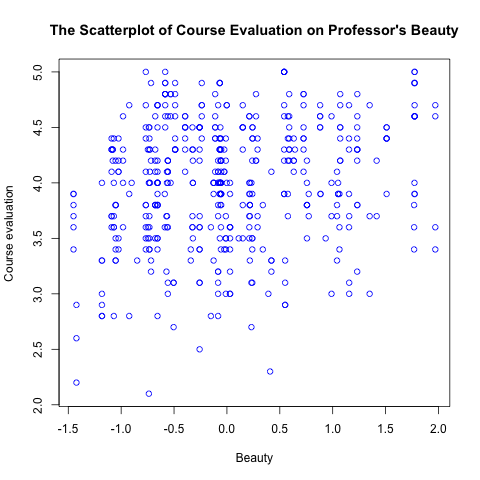
\includegraphics[width=0.75\textwidth]{beauty.png}
\caption{\label{fig:org2c95145}
The scatterplot of course evaulation on professors' beauty}
\end{figure}


\subsection*{Regression}
\label{sec:org80f26a9}

Now let's estimate the regression model. The results is reported
in Table \ref{tab:ols-1}

\begin{verbatim}
# run a regression of course evaluation on professor's beauty
teaching.ols <- lm(teaching.formula, data = teachingdata)

# create the latex table
stargazer(teaching.ols,
  covariate.labels = c("Beauty"),
  dep.var.labels = c("Course Evaluations"),
  title = "The OLS Estimation of the Regression of Course Evaluation on Beauty",
  label = "tab:ols-1", single.row = TRUE, omit.stat = c("adj.rsq", "f")
)
\end{verbatim}


% Table created by stargazer v.5.2 by Marek Hlavac, Harvard University. E-mail: hlavac at fas.harvard.edu
% Date and time: Wed, Apr 05, 2017 - 20:21:26
\begin{table}[!htbp] \centering
  \caption{The OLS Estimation of the Regression of Course Evaluation on Beauty}
  \label{tab:ols-1}
\begin{tabular}{@{\extracolsep{5pt}}lc}
\\[-1.8ex]\hline
\hline \\[-1.8ex]
 & \multicolumn{1}{c}{\textit{Dependent variable:}} \\
\cline{2-2}
\\[-1.8ex] & Course Evaluations \\
\hline \\[-1.8ex]
 Beauty & 0.133$^{***}$ (0.032) \\
  Constant & 3.998$^{***}$ (0.025) \\
 \hline \\[-1.8ex]
Observations & 463 \\
R$^{2}$ & 0.036 \\
Residual Std. Error & 0.545 (df = 461) \\
\hline
\hline \\[-1.8ex]
\textit{Note:}  & \multicolumn{1}{r}{$^{*}$p$<$0.1; $^{**}$p$<$0.05; $^{***}$p$<$0.01} \\
\end{tabular}
\end{table}



\subsection*{Answers to the questions}
\label{sec:orgaf7e57c}

\begin{description}
\item[{a.}] The scatterplot is Figure \ref{fig:org2c95145}. There appears to be
a weak positive relationship between course evaluation and the
beauty index.

\item[{b.}] The estimation results are reported in Table \ref{tab:ols-1}.

\begin{verbatim}
beauty.watson <- mean(teachingdata$beauty)
beauty.stock <- mean(teachingdata$beauty) + sd(teachingdata$beauty)
ave.courseval <- mean(teachingdata$course_eval)

# do prediction step by step
b0 <- teaching.ols$coef[1]
b1 <- teaching.ols$coef[2]
courseval.predict <- b0 + b1 * c(beauty.watson, beauty.stock)
names(courseval.predict) <- c("waston", "stock")
\end{verbatim}

The slope is \texttt{0.133} and the intercept is
\texttt{3.998}. The sample mean of course evaluation is
\texttt{3.998}, which coincides with the slope
because the sample mean of \emph{Beauty} is
\texttt{0}.
\end{description}


\begin{description}
\item[{c.}] The beauty indices for Professors Stock and Watson are
\texttt{0.7886} (one standard deviation)
and \texttt{0} (sample average).
Thus, the predicted course evaluations for Professors
Stock and Watson are \texttt{4.1032} and
\texttt{3.9983}, respectively.

\begin{verbatim}
beauty.sd <- sd(teachingdata$beauty)
courseval.sd <- sd(teachingdata$course_eval)
delta.courseval <- b1 * beauty.sd
\end{verbatim}

\item[{d.}] The standard deviation of course evaluation is
\texttt{0.5549}, and the standard deviation of
beauty is \texttt{0.7886}. A one-standard-deviation
increase in beauty is expected to increase course evaluation
by \texttt{0.1049}, or
\texttt{0.19} of standard deviation of course
evaluations. The effect is small.

\begin{verbatim}
rsq <- summary(teaching.ols)$r.squared
\end{verbatim}

\item[{e.}] The regression R\(^{\text{2}}\) is \texttt{0.0357}, so that \emph{Beauty}
explains only \texttt{3.6} percent of the
variance in course evaluations.
\end{description}
\end{document}